\documentclass[border=3pt]{standalone}
\usepackage{tikz}
\usetikzlibrary{decorations.pathreplacing,patterns}
\definecolor{greengreen}{rgb}{0.0, 0.42, 0.24}
%%%%%%%%%%%%%%%%%%%%%%%%%%%%%%%%%%%%%%%%%%%%%%%%%%%%%%%%%%%%%%%%%
\begin{document}
%%%%%%%%%%%%%%%%%%%%%%%%%%%%%%%%%%%%%%%%%%%%%%%%%%%%%%%%%%%%%%%%%
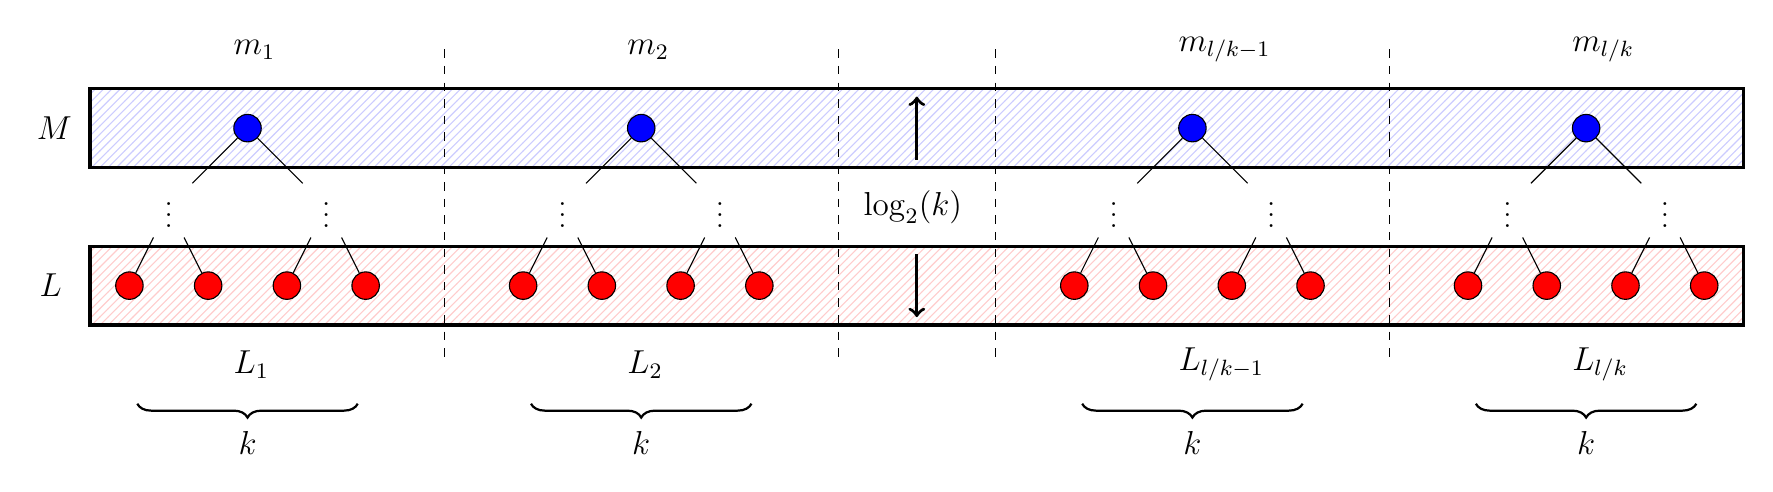
\begin{tikzpicture}[every node/.style={align=center},
red/.style={fill=red,draw,circle,inner sep=0pt},
blue/.style={fill=blue,draw,circle,inner sep=0pt},
 text width = .35cm]
%================================================================
%	Boxes
\draw[very thick, pattern=north east lines, pattern color=red!20] (-0.5,-0.5) rectangle (20.5,0.5);
\draw[very thick, pattern=north east lines, pattern color=blue!20] (-0.5,1.5) rectangle (20.5,2.5);

%================================================================
%	Nodes
\node[style=red] (r1) at (0,0) {};
\node[style=red] (r2) at (1,0) {};
\node[style=red] (r3) at (2,0) {};
\node[style=red] (r4) at (3,0) {};
\node[style=red] (r5) at (5,0) {};
\node[style=red] (r6) at (6,0) {};
\node[style=red] (r7) at (7,0) {};
\node[style=red] (r8) at (8,0) {};
\node[style=red] (r9) at (12,0) {};
\node[style=red] (r10) at (13,0) {};
\node[style=red] (r11) at (14,0) {};
\node[style=red] (r12) at (15,0) {};
\node[style=red] (r13) at (17,0) {};
\node[style=red] (r14) at (18,0) {};
\node[style=red] (r15) at (19,0) {};
\node[style=red] (r16) at (20,0) {};
%----------------------------------------------------------------
\node (d1) at (0.5,1) {$\vdots$};
\node (d2) at (2.5,1) {$\vdots$};
\node (d3) at (5.5,1) {$\vdots$};
\node (d4) at (7.5,1) {$\vdots$};
\node (d5) at (12.5,1) {$\vdots$};
\node (d6) at (14.5,1) {$\vdots$};
\node (d7) at (17.5,1) {$\vdots$};
\node (d8) at (19.5,1) {$\vdots$};
%----------------------------------------------------------------
\node[style=blue] (b1) at (1.5,2) {};
\node[style=blue] (b2) at (6.5,2) {};
\node[style=blue] (b3) at (13.5,2) {};
\node[style=blue] (b4) at (18.5,2) {};

%================================================================
%	Lines
\draw (r1) -- (d1);
\draw (r2) -- (d1);
\draw (r3) -- (d2);
\draw (r4) -- (d2);
\draw (r5) -- (d3);
\draw (r6) -- (d3);
\draw (r7) -- (d4);
\draw (r8) -- (d4);
\draw (r9) -- (d5);
\draw (r10) -- (d5);
\draw (r11) -- (d6);
\draw (r12) -- (d6);
\draw (r13) -- (d7);
\draw (r14) -- (d7);
\draw (r15) -- (d8);
\draw (r16) -- (d8);
%----------------------------------------------------------------
\draw (d1) -- (b1);
\draw (d2) -- (b1);
\draw (d3) -- (b2);
\draw (d4) -- (b2);
\draw (d5) -- (b3);
\draw (d6) -- (b3);
\draw (d7) -- (b4);
\draw (d8) -- (b4);
%----------------------------------------------------------------
\draw[dashed] (4,3) -- (4,-1);
\draw[dashed] (9,3) -- (9,-1);
\draw[dashed] (11,3) -- (11,-1);
\draw[dashed] (16,3) -- (16,-1);

%================================================================
%	Decoration
\draw[thick, decorate,decoration={brace,amplitude=5pt,mirror}] (0.1,-1.5) -- (2.9,-1.5);
\draw[thick, decorate,decoration={brace,amplitude=5pt,mirror}] (5.1,-1.5) -- (7.9,-1.5);
\draw[thick, decorate,decoration={brace,amplitude=5pt,mirror}] (12.1,-1.5) -- (14.9,-1.5);
\draw[thick, decorate,decoration={brace,amplitude=5pt,mirror}] (17.1,-1.5) -- (19.9,-1.5);

\draw[->, very thick] (10, 1.6) -- (10, 2.4);
\draw[->, very thick] (10, 0.4) -- (10, -0.4);
\node at (9.5,1) {\large $\log_2(k)$};
%----------------------------------------------------------------
\node at (-1,2) {\large $M$};
\node at (-1,0) {\large $L$};
%----------------------------------------------------------------
\node at (1.5,3) {\large $m_1$};
\node at (6.5,3) {\large $m_2$};
\node at (13.5,3) {\large $m_{l/k-1}$};
\node at (18.5,3) {\large $m_{l/k}$};
%----------------------------------------------------------------
\node at (1.5,-1) {\large $L_1$};
\node at (6.5,-1) {\large $L_2$};
\node at (13.5,-1) {\large $L_{l/k-1}$};
\node at (18.5,-1) {\large $L_{l/k}$};
%----------------------------------------------------------------
\node at (1.5,-2) {\large $k$};
\node at (6.5,-2) {\large $k$};
\node at (13.5,-2) {\large $k$};
\node at (18.5,-2) {\large $k$};
%================================================================
\end{tikzpicture}
%%%%%%%%%%%%%%%%%%%%%%%%%%%%%%%%%%%%%%%%%%%%%%%%%%%%%%%%%%%%%%%%%
\end{document}
%%%%%%%%%%%%%%%%%%%%%%%%%%%%%%%%%%%%%%%%%%%%%%%%%%%%%%%%%%%%%%%%%